\section{Implementation}

\subsection{About Ngene}
\emph{Ngene} is a flexible, generic, multi-purpose genetic algorithm engine written in C++ with heavy emphasis on performance and flexibility. The engine is divided into logical modules that can be interchanged or extended upon in order to fit the intended goal.

The prototype for this engine started out as an assignment for a sub-symbolic artificial intelligence course. It was written in Python, which later proved to be too slow for this kind of application, and later partially ported to C++ because I wanted to learn the language at the time. The engine was finally picked up again, and completed for the purpose of this thesis.

\subsubsection{Modular Design}
The design is broken into the following modules:

\begin{itemize}
	\itemsep=0pt
	\item (core) - The genetic algorithm itself
	\item Fitness - Assesses the fitness of a genotype
	\item Genotype - Produces the genotype and translates them to phenotype
	\item Mating - Crosses two genotypes
	\item Mutator - Mutates a genotype
	\item Selector - Selects a random genotype
\end{itemize}

All modules are loaded into memory when the program is executed and kept there until the program is terminated. This modular design is essential when it comes to making the engine available for all purposes. For example, while \emph{tournament} selection is suitable for most of the experiments in this thesis, other users may want to run a comparison test between different selection methods. This is easily achieved by simply specifying which module to use in a configuration file. There is no need to recompile a single line of code unless a new module is required. This modular design also keeps the code cleaner and easier to maintain.

\subsubsection{Why C++?}
In a sense, one can say that this project was made possible because of my prototype in Python. It taught me many higher level concepts that is practically non-existant in lower level languages such as C++. Without it, I probably wouldn't have been able to bring the project to the level it is today. Especially without the concept of a dynamic type, the idea of a container that can contain anything from an integer, to a string, to a floating type number, I would still have trouble trying to compensate for it with complex algorithms to deal with raw data pointers. Most importantly, it taught me the importance of optimization and use of libraries.

Choosing a programming language depends on what kind of application you want to write. A simple program with no special requirements can be written in any language. For instance, a mail client written in Python will perform equally well as any other client because the focus lies on fetching and displaying e-mails and the ability to manage them in a clear way. The features are more important than the extra two milliseconds it takes to perform a query. However, there are applications for which performance is more important than anything. Arguably, such programs should be written in one of two ways: In assembly (or machine code) or C/C+. While assembly is rarely used these days, due to being practically unreadable for mortals, C and C++ is often used for time critical applications. Unlike languages that depend on a virtual machine (C\#, Java), or an interpreter (Common LISP, Python), code written in C/C++ is compiled directly to machine code before executed, often yielding much better performance.

C++ is thought of as being a middle level language: It has the advantages of both the lower (machine code) and higher level languages, but also the inherent disadvantages. For example, all memory management must be explicitly handled in the code because C++ lacks a garbage collection found typically in C\# or Java. This means that we have to be careful of memory leaks and access of invalid memory addresses. Failure to do so may cause a huge performance hit. Furthermore, C++ doesn't come with as big a convenience library as those found in aforementioned languages. Such a library would eliminate rewriting often used algorithms and the headache of fixing a buggy code. Fortunately, efforts are already being made to ease the implementation through external libraries.

\subsubsection{Boost C++ Libraries}
\emph{Boost}\footnote{\url{http://www.boost.org/}} is a collection of libraries which complement the C++ Standard Library (STL). Ngene makes use of this collection, saving time and effort, and guaranteeing that such code works as it should.

\paragraph{\textbf{Boost.Any}}\cite{henney2001}
A problem with writing a generic genetic algorithm in a strongly typed programming language such as C++, is that different studies require different data types to be passed around the system. A simple program that sorts numbers, for instance, needs to pass around an array with integers while another one may require the use of a class or custom data type. In a higher level language such as Python, a container is already available that can store any type of data:

\begin{verbatim}
>>> foo = 1 + 2
>>> print foo
3
>>> foo = "awesome"
>>> print foo
awesome
>>> _
\end{verbatim}

Fortunately, this has already been implemented and is freely available as part of \emph{Boost}. The modular design would otherwise not work without, at least not within given time constraint. \emph{Boost.Any} is a container not very different from the one found in Python and only requires a type-casting before the data can be handled as normal.

\paragraph{\textbf{Boost Random Number Library}}\cite{maurer2000}
Another problem with genetic algorithms and development in general is implementing a good pseudo-random number generator. Ngene uses the implementation of \emph{Mersenne twister} pseudo-random number generator found in the Boost libraries. This generator was chosen for its long period ($2^(19937) - 1$ to be exact), and because it is relatively fast compared to other algorithms. It also passes a number of tests for randomness, including Diehard\footnote{A collection of tests to measure the quality of the randomness of the generator, developed by George Marsaglia.} and most of the TestU01 Crush randomness tests.

\subsubsection{Brief System Overview}
\begin{figure}[!ht]
	\centering
	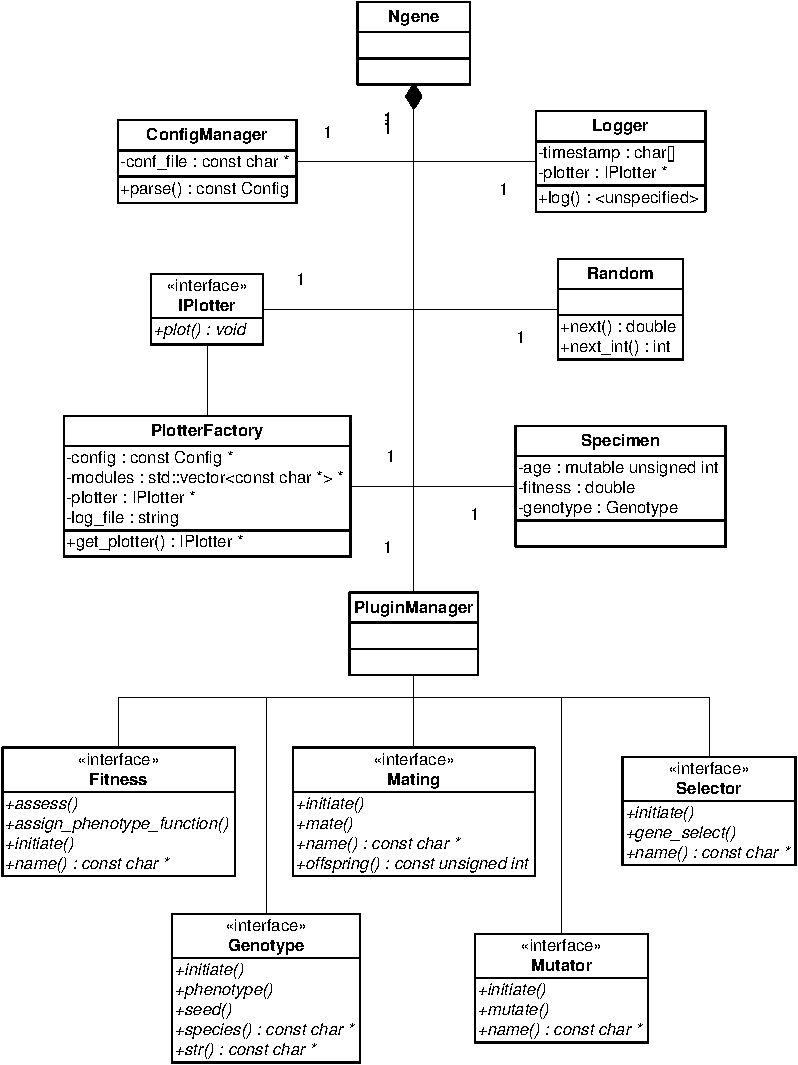
\includegraphics[scale=0.9]{diagram_ngene}
	\caption{Overview of Ngene}
	\label{fig:diagram_ngene}
\end{figure}

Figure~\ref{fig:diagram_ngene} shows a brief overview of how Ngene is put together. At startup, three of these parts are responsible for what must happen before anything can be run in accordance with the user's parameters. \texttt{ConfigManager} takes care of reading the configuration file and makes sure that all other parts have access to and will understand what it is told to do. Once it has played its part, \texttt{PluginManager} should be able to load relevant modules and \texttt{Logger} will know whether or not it should plot a fitness/generation graph of a population or just write some text to a file.

The genetic algorithm is very simple:
\begin{enumerate}
	\itemsep=0pt
	\item An initial population is randomly generated.
	\item \texttt{Specimen}s are randomly selected for crossover.
	\item Repeat step 2 until the offspring population is of satisfactory size.
	\item Replace adult population with offspring population.
	\item Repeat process from step 2 until the maximum number of generations is reached, or a perfect \texttt{Specimen} is found.
	\item Write log/graph and final \texttt{Specimen} to disk.
\end{enumerate}

The final step is the responsibility of \texttt{Logger}. \texttt{Logger} has no knowledge of what format the \texttt{Specimen} should be written as. Be it a text file, an image or a proprietary format, it will simply request the \texttt{Genotype} module to give it some data to write to disk. The output format is actually hard-coded into each \texttt{Genotype} module. Because this rarely changes for a single experiment and/or model, otherwise a new module must be written anyway, this has no real impact on users.

\texttt{PluginManager}, along with the responsibilities of loading and releasing modules, will also act as a layer between the modules and the algorithm itself. The engine will never have to bother with the specifics of each module, but rather be able to just tell what a module ought to do. Of course, this requires that the modules follow certain specifications in order to be compatible with this layer. These are described in more detail in the system documentation for Ngene.


\subsection{Ngene Development Framework}
\begin{figure}[!ht]
	\centering
	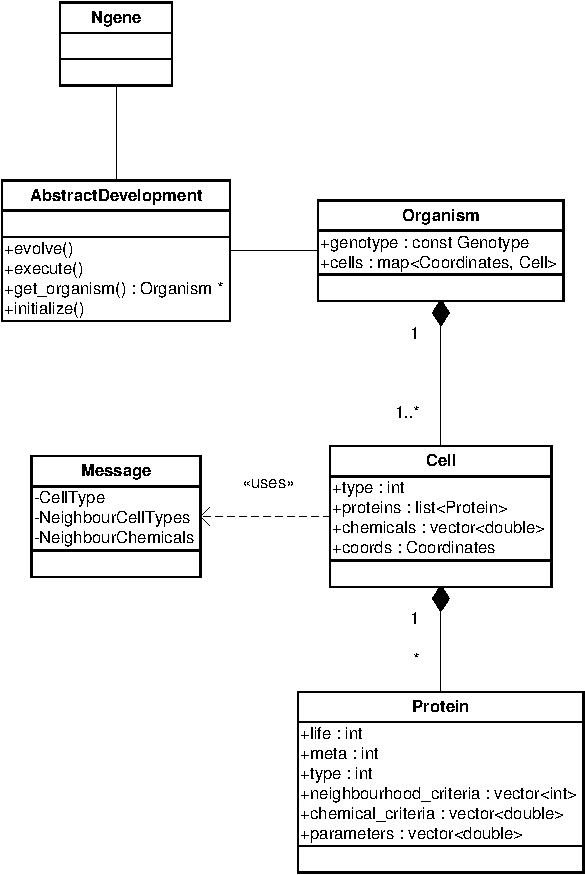
\includegraphics[scale=0.9]{diagram_ndevframe}
	\caption{Overview of Ngene Development Framework}
	\label{fig:diagram_ndevframe}
\end{figure}

As it stood, Ngene gave the users too much freedom in implementing their own modules, making it difficult to compare two models without having to factor in differences in implementations. A generic development framework was therefore devised to eliminate these factors and ease the implementation at the same time. The framework was designed to accommodate any conceivable model.

The framework provides a code base that implements a common development algorithms, along with common concepts such as a cell or a protein (see fig.~\ref{fig:diagram_ndevframe}). This includes intercellular communication (see fig.~\ref{fig:diagram_ndevframe_msg}) and development stepping in order to reduce any implementation advantages a model has over another. Use of this code base is enforced in order to ensure that all comparison made between different development models will be based on a common ground.

\begin{figure}[!ht]
	\centering
	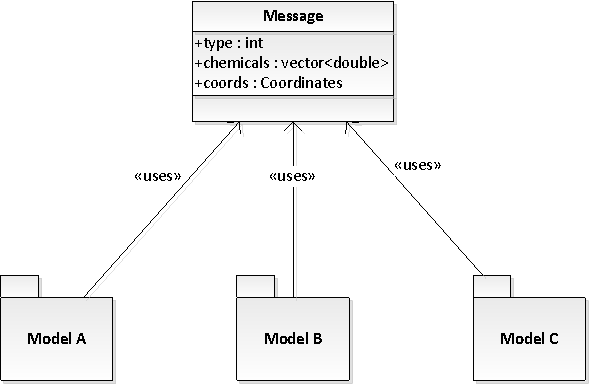
\includegraphics[scale=0.9]{diagram_ndevframe_msg}
	\caption{A common message implementation should eliminate factors involving what information is exchanged between the organism's cells.}
	\label{fig:diagram_ndevframe_msg}
\end{figure}

Figure~\ref{fig:diagram_ndevframe_common-base} shows three different scenarios where model A and B use only chemicals, while model C only makes use of proteins. This tells us that model A and B may use both the cell type and the chemicals part of a \texttt{Message}, while model C only takes cell type into consideration (or it may not even make use of communication). We also see that model B and C make use of a control program besides the genome. Even though these three models are different, they still use the same framework or code base. A comparison can then be performed without having to take into account implementation differences that may affect one model or another.

\begin{figure}[!ht]
	\centering
	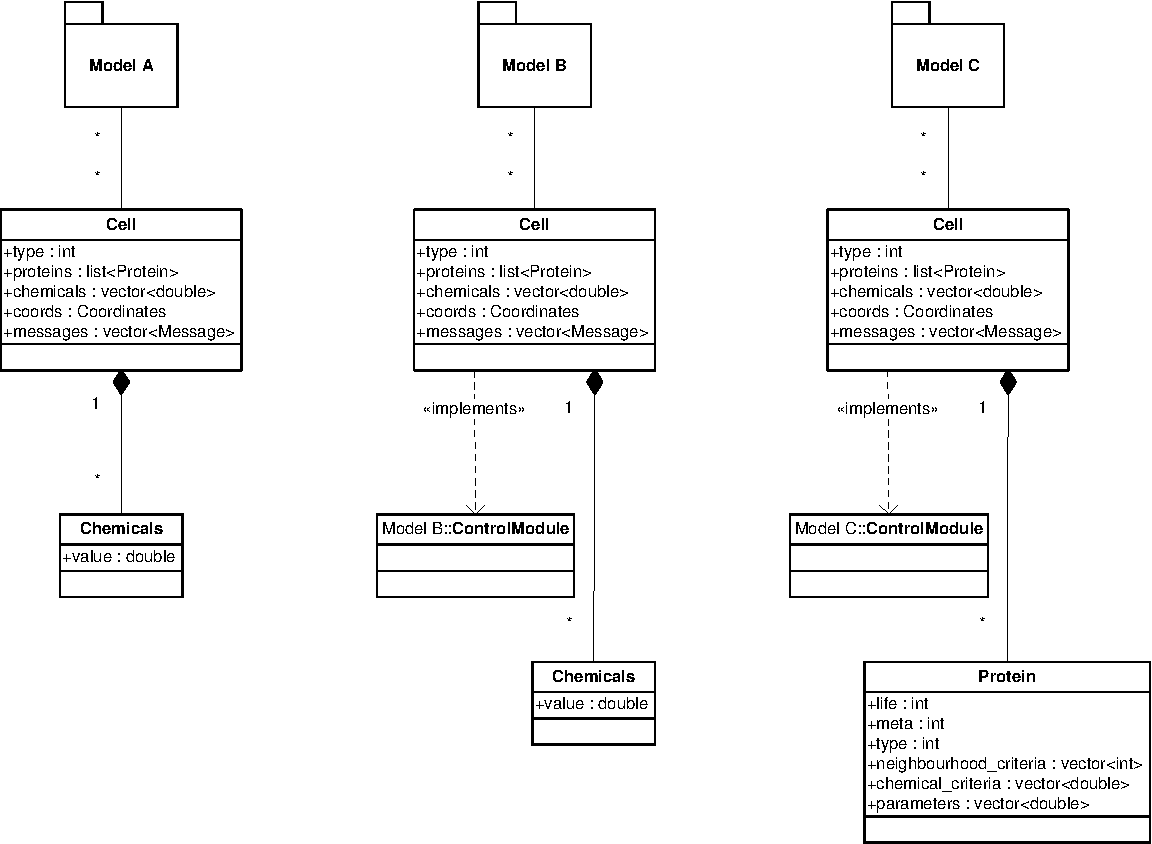
\includegraphics[scale=0.8]{diagram_ndevframe_common-base}
	\caption{Albeit different, all three models still use the same implementation of a cell, chemicals and proteins, and receive the same messages.}
	\label{fig:diagram_ndevframe_common-base}
\end{figure}

With regards to speed optimizations, lots of thought as been put into how to represent the organisms themselves. In the current implementation, a C++ Standard Library (STL) \texttt{<map>} is used to store the cells using their coordinates as the key value. Other alternatives were also considered:

\begin{center}
	\begin{tabular}{ r | c | c | c }
		~ & STL \texttt{<map>} & STL \texttt{<vector>} & STL \texttt{<ext/hash\_map>} \\
		\hline
		element access & $O(log~n)$ & $O(1)$ & $O(1)$ \\
		\hline
		insertion & $O(log~n)$ & $O(1)$ & $O(1)$ \\
		\hline
		search & $O(log~n)$ & $O(n)$ & $O(1)$ \\
	\end{tabular}
	\label{tbl:speed}
\end{center}

A quick glance at the comparison table and the \texttt{<ext/hash\_map>} may seem like the best choice to go with. However, there are some drawbacks that must be taken into consideration. A good hashing algorithm is essential for the performance of the hash table by providing a uniform distribution over the array. Too simple, and a lot of collisions will occur, but too complex and the hashing table will spend all of its time calculating a hash value. Collisions occur regardless of how good the algorithm is. The \emph{birthday paradox} predicts that it doesn't take many elements before the chance of a collision exceeds 95\%, even for very big arrays. A good collision resolution is therefore also needed but will not be enough to guarantee the performance advantage over other solutions. For the experiments conducted in this thesis, the number of cells rarely exceeded 1000. For a \texttt{<map>}, this means at most 10 comparisons to find an element by its key value. A hash table would require about the same number of operations to calculate the hash, perform the lookup and resolve any collisions.

The \texttt{<map>} was chosen over the \texttt{<vector>} because despite its better access and insertion times, required more time to find all of a cell's neighbours. This can be remedied by creating and maintaining a neighbours list for every cell. However, this would make insertion $O(n)$ as opposed to $O(log~n)$ of the \texttt{<map>}.

\subsubsection{Using the Framework}
\begin{figure}[!ht]
	\centering
	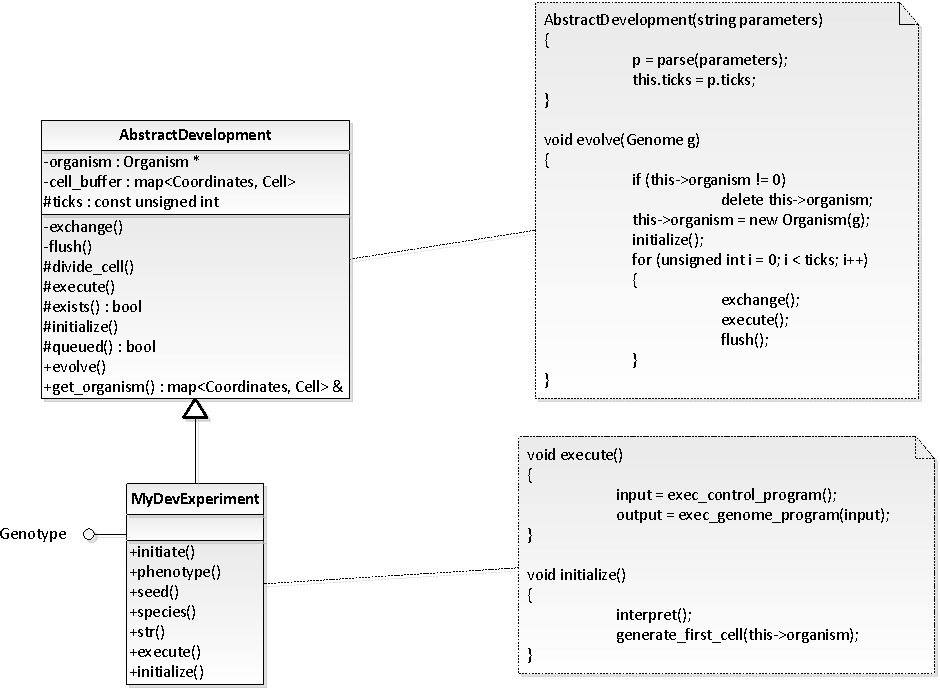
\includegraphics[scale=0.9]{diagram_ndevframe_ex}
	\caption{An example of how one can implement \texttt{MyDevExperiment}.}
	\label{fig:diagram_ndevframe_ex}
\end{figure}

The framework was designed to ease the implementation effort as much as possible. The whole code base can be inherited from \texttt{AbstractDevelopment} (see fig.~\ref{fig:diagram_ndevframe_ex}). To make it your own module, only two functions need to be implemented, \texttt{execute()} and \texttt{initialize()}. The latter is executed once with every new organism that is to be developed, and can be used to unpacking the genotype to a cellular program and/or generating initial cells in the organism. The \texttt{execute()} function is called every development step/tick, for every cell in the organism. Here, the cell program from the genotype can be executed as well as any control programs that might be needed. Note that any messages sent has already been received and are stored in the cells themselves by the time a cell is given the chance to fulfil its purpose in a tick. It will not be possible to actually access the organism itself from this function in order to avoid accidental tampering.

For the purpose of this thesis, two models were implemented within this framework not only to test the flexibility and performance of this framework but also to see what is missing and what areas need improvement.

\subsubsection{ArtDev3D}
Porting Johan H{\o}ye's master's thesis\cite{hoye2006} to Ngene's framework was a rather cumbersome job, partly due to little system documentation and partly because many biology concepts made their way into his code. Porting this code to Ngene's framework has been a matter of finding out what occurs in a cell during a development step, and whether or not there are external processes that needs to be accounted for. As described in \ref{sec:ArtDev3D}, the innards of the cell perform


TODO


The hierarchy of the system runs very deep, ie. a single function may need to call other functions which call different functions, and so on, in order to perform simple cellular operations. This makes it hard to follow the flow of the code and may have a negative impact on performance. A single cell may call this function several times in a single tick, and there are many cells in a single organism, not to mention an entire population over many generations. Reducing the number of function calls will also reduce any potential strain on the call stack, and in turn better the performance. Efforts has therefore been made to flatten the structure and simplify as much as possible without comprimising the logical integrity of the model. In addition to some fresh documentation, it will hopefully make it even easier to understand.

There is an issue that has been addressed with the porting of this model, and may therefore offer different results than the original. In most models, cells are developed simultaneously. Before a cell can execute its functions, information must be exchanged between all cells so that when it is run, it will base its operations on the current state and not the updating one. In ArtDev3D, this is not properly implemented. This concern points to a couple of lines of code that perform a single development step inside the cell. Upon execution, the cell will start collecting requests from its proteins. The proteins can request an action when they are activated, i.e. when the state of the cell and its neighbours are above a threshold. The requests are queued up and then executed. The problem with this, is that it all happens in a single step. Thus, cells that already have had their turn before the current cell, will have an altered state. Actions are therefore based on a mix of ``newer'' information from these cells, and ``old'' information from the rest. When porting this code to the new framework, the cell will no longer have direct access to other cells. Instead, it will receive messages from (or a snapshot of) nearby cells before the development step takes place in any cell.

\subsubsection{Cartesian}
This model is based on a number of works by Julian F. Miller, mainly \cite{mteurogp2000} and \cite{ecal2003}. 

TODO

Mutation upwards has an impact
Implement bit check error

\subsubsection{Performance}

TODO

